\chapter{Introduction}

% Introduction to the internet, data, basic text representations
% Introduction to machine learning, benefits of data for machine learning, machine learning representations
% Problems with machine learning, interpretability, lack of interpretability in machine learningg
% We introduce a series of methods for transforming uninterpretable machine learning representations into interpretable ones
% Finding directions in vector spaces and using those to produce interpretable representations
% Fine-tuning these directions to get a better result
% Interpreting and investigating neural networks with these directions


Smartphones and other devices that keep people connected to the internet are prevalent, resulting in a deluge of publicly available data. In particular, applications that enable user-generated content e.g. Social Media sites (Facebook, Twitter), Review sites (IMDB, Rotten Tomatoes, Amazon) and content-aggregation sites (Reddit, Tumblr) produce a lot of text data e.g. in posts and comments. Research into how it can be used to solve a variety of problems has been conducted, e.g. using text data to identify if social media posts, or product reviews, are positive or negative \cite{Burel2018}, to identify social media posts that happen during crises and identify those that are useful to crisis responders \cite{Burel2018}, or even to predict depression in social media users \cite{Aldarwish2017}. 

The methods to solve these problems are a result of machine-learning, which uses a large amount of data to learn how to solve some specific problem. Machine-learning is a force that has began to take-part in our day-to-day interactions with both the online and offline space, in the online world through content recommendation, targeted marketing and advertisement, and a variety of businesses that have sprung up with some machine-learning tool at the center. In the offline world, self-driving cars, face recognition on CCTV, behaviour prediction of crowds among others have started taking place across the world. Essentially, these tools are able to succeed because of the availability of data.

Problems that machine-learning can solve can be split into two distinct categories, supervised and unsupervised. Supervised problems have some data that is labelled, and some that is not labelled. The goal of a supervised task is to assign labels to the data that is not labelled, by learning with the data that is labelled. Unsupervised problems do not have any labels, and instead try to solve a problem just from unlabelled data. The learning method to solve the problem is called a machine-learning model. In a supervised task this model  learns using the labelled examples, and then is used to label the unlabelled examples.

One example of an unsupervised machine-learning task is to transform data into a representation that can be learned from by the 

\section{Motivation}
%What is text? How is it motivating?

%What are the desiradata of a good representation?
% Unsupervised


One task of Natural Language Processing is to obtain this semantic understanding from text by obtaining a machine-readable representation that contains domain knowledge. A basic approach to obtain a representation of this text is to represent entities (e.g. reviews, text-posts) by the frequency of their words, see \ref{Bag-of-words-example}.

\begin{figure}[t]
	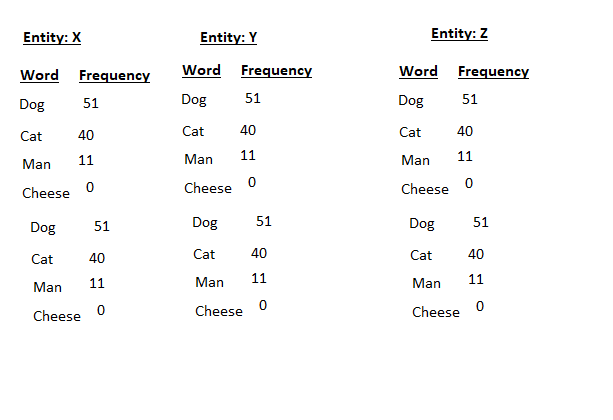
\includegraphics[width=\textwidth]{images/bowbowbow.png}
	\centering
	\caption{Bag-of-words  }\label{Bag-of-words-example}
\end{figure}


 Below, we show a review with its associated properties labelled.

\begin{figure}[t]
	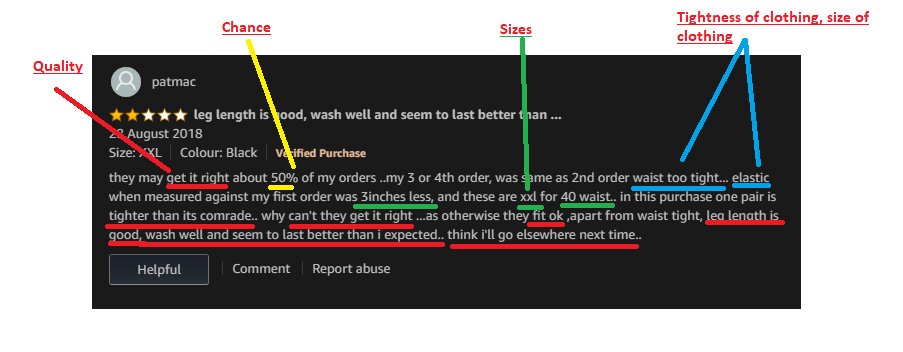
\includegraphics[width=\textwidth]{images/leg_length.png}
	\centering
	\caption{Example properties  }\label{IntroDecisionTree}
\end{figure}

\subsection{Machine Learning}
% what is machine learning? why do i care?


% Granular
We can understand these properties to have a degree to which they apply, for example the size of the clothing might be "XXL", "XL", "L", "M" or "S", or the quality may be "Very good", "Good", "Ok", "Bad" or "Very bad". For the former, we may rely on the metadata available from the site itself, but for the latter the way to obtain this information is less clear. Although we may infer that the rating has some indication of these properties, it does not describe the properties or the degree to which the review refers to them. This kind of information is valuable for making sense of the world of unstructured text, and has broad applications, e.g. The most immediate example is perhaps that they allow for a natural way to implement critique-based recommendation systems, where users can specify how their desired result should relate to a given set of suggestions \cite{viappiani2006preference}. For instance, \cite{Vig:2012:TGE:2362394.2362395} propose a movie recommendation system in which the user can specify that they want to see suggestions for movies that are ``similar to this one, but scarier''. If the property of being scary is adequately modelled as a direction in a semantic space of movies, such critiques can be addressed in a straightforward way. Similarly, in \cite{kovashka2012whittlesearch} a system was developed that can find ``shoes like these but shinier'', based on a semantic space representation that was derived from visual features. Semantic search systems can use such directions to interpret queries involving gradual and possibly ill-defined features, such as ``\emph{popular} holiday destinations in Europe'' \cite{DBLP:conf/sigir/JameelBS17}. While features such as popularity are typically not encoded in traditional knowledge bases, they can often be represented as semantic space directions.  %Copied from CONLL

\subsection{Directions}\label{intro:directions}


However, manually labelling these properties and the degrees to which entities (e.g. reviews, text-posts) have them is extremely time-consuming. 

A potentially ideal system would be as follows: We collect large amounts of unstructured text data, separated into domains, and obtain the properties of each domain from this data, and rank entities on the degree to which they have these properties. In this way, properties would be understood on a scale built from the domain directly, so that each domain has its own meanings for words according to their own idiosyncrasies. As the process does not require any manual labelling the quality of these properties could be improved simply by obtaining more data. Further, as we are learning from unstructured data, not only would this allow us to understand the data in terms of what we know, but it would also introduce us to new ideas that we may not have previously understood. This kind of representation also has value in application to Machine Learning tasks. If we can separate the semantics of the space linearly into properties, we are able to learn simple linear classifiers that perform well. 

Simple linear classifiers built from a representation composed of rankings on properties have an additional benefit of being more understandable.


% Natural clustering
% Semantically distinct
% Interpretable
% Curse of dimensionality
% Generalizability ("shared factors across many tasks" \cite{Bengio2012})

%What is machine learning? What are its advantages? How is it motivating?

%What are the problems with machine learning? How is it motivating?


%What is domain-specific? What is domain knowledge? %On the web there is a large volume of raw text data, e.g. Reviews of products, movies, anime, books, music, social posts by individuals, self-descriptive text about a website or product, and so on. These can be categorized into domains; each domain has its own quirks, knowledge, and method of being brought about. Although a movie review may sound similar to a book review, they typically differ hugely in the distribution of words used.

%

\section{Interpretability}\label{ch1:interpret}

%What is interpretability? How is the value of interpretability measured in the real world?

%How can we meet the needs of the real world?  Is it transparancy, the system having easy to understnad components, etc... what  are the different views on what an interpretabile system is?

%What specific interpretability task are we trying to solve? How do we define interpretability? Why is it valuable, where is it used? What was the hypothesis/research question?
%%What are distributional models?
Most successful approaches in recent times, like vector-spaces, word-vectors, and others, rely on the distributional model of semantics. This model relies on encoding unstructured text e.g. of a movie review, as a vector, where each dimension corresponds to how frequent each word is, we are able to calculate how similar the entities are, e.g. we know that if two movies have a similar distribution of words in their reviews, like frequent use of the word 'scary', or 'horror', then they would have a higher similarity value. These models, also known as 'semantic spaces' encode this similarity information spatially.

Semantic relationships can be obtained from semantic spaces. 

applications/need for good interpretability:
\begin{itemize}
	\item Safety
	\item Troubleshooting, bug fixing, model improvement
	\item Knowledge learning
	\item EU's "Right to explanation"
	\item Discrimination
\end{itemize}

%What is a conceptual space? What are entities?  What are properties? What is commonsense reasoning?
properties of an interpretable classifier:
\begin{itemize}
	\item Complexity: 'the magic number is seven plus or minus two' \cite{Saaty2003} also has many positive effects for its users, like lower response times \cite{Narayanan2018, Huysmans2011}, better question answering and confidence for logical problem questions \cite{Huysmans2011} and higher satisfaction \cite{Narayanan2018}.
	\item Transparancy: 
	\item Explainability: 
	\item Generalizability:
\end{itemize}


%X%X%What is a symbolic approach?  %One approach to making sense of these domains is to produce rules from expert knowledge. An expert in movies would tell you that if the review talks about it being a "cannibal horror film", we can understand that it is likely a scary movie and is related to the original 'Cannibal Holocaust' movie. Encoding this kind of knowledge is difficult, time-consuming, and hard to automate reliably.

Properties, entities, the benefits and application of a representation formed of these

Basic introduction to directions, explanation of the utility and application of our approach
\section{Thesis Overview / Contributions}

%What were our objectives starting out? 
%What are our intentions with how the work in the thesis will be used?
%What are our contributions?
%%What are our aims for this chapter? What do we overall want to do? (Already kind-of said in Chapter 1, but worth repeating I guess in some form)
%In \ref{Chapter3}, we introduce a pipeline that starts with unstructured text, and ends with an interpretable representation of entities represented by properties labelled by clusters of words. Further, we demonstrate the applicability of these representations in a simple Decision Tree that uses just a few of these properties to classify entities. In Figure \ref{ExamplesWithTree}, we show some example movie entities, their associated properties, and a Decision Tree classifying whether or not they are a Horror movie. 

In \ref{Chapter3}, we focus on further experimenting with one relationship that was formalized in \cite{Derrac2015}: a ranking of entities on properties. In particular, we use this method of building a representation of entities as a way to convert a vector space into an interpretable representation, for use in an interpretable classifier. The reason that we chose this representation to expand on is because by representing each entity $e$ with a vector $v$ that corresponds to a ranking $r$, the meaning of each dimension is distinct, and we are able to find labels composed of clusters of words for these dimensions. Here, we make the distinction between a property and a word, a property is a natural property of the space that exists in terms of a ranking of entities, and words are the labels we use to describe this property.